% !TeX spellcheck = en_US
\addscenariosection{1}{Cooperative Scenario}{Close to enemies}{\images/balistic.png}

\begin{multicols*}{2}

\textbf{Author:} Kelghor

\textbf{Version:} 1.4

\textbf{Source:} \href{https://discord.com/channels/740870068178649108/1313651865648369725}{Archon Studio Discord}

\textit{"Sir! They're here again!"}

\textit{"Sound the alarm, we'll repel them as always!" you command, and go to defend the city, just as you have done many times before. Such is the hard life of the surrounding clans, with constant wars and skirmishes with nearby neighbors. Fortunately, your alliance is strong, so you know your back is covered.}

\textit{Therefore, the time has come to end the long-standing wars and crush your enemies once and for all!}

\subsection*{\MakeUppercase{Scenario Length}}

This Scenario is played over 7 Rounds.

\subsection*{\MakeUppercase{Player Setup}}

\textbf{Player Count:} 1-6

\textbf{Starting Resources:} 14 \svg{gold}, 5 \svg{building_materials}, 2 \svg{valuables}

\textbf{Starting Income:} 10 \svg{gold}, 2 \svg{building_materials}, 0 \svg{valuables}

\textbf{Starting Units:}
\begin{itemize}
  \item  1 × A Few \svgunit{bronze} Units of your choice
\end{itemize}

\textbf{Town Buildings:} \svgunit{bronze} Dwelling.

\textbf{Additional Bonus:}: Only base bonus by difficulty (see the main rules).

\textbf{Map Tile Pool:} Take $P$ × random Far (II–III) map tiles as shared pool. None of them must contain a settlement. ($P$ stands for the number of players)

\subsection*{\MakeUppercase{Map Setup}}

Take the following Map Tiles and arrange them as shown in the Scenario map layout.
Setup Far (II--III) Map Tiles with settlements of same Faction as players Towns as show a color cube, or see example.

\begin{itemize}
  \item $P$ × Starting (I) Map Tile.
  \item $P$ × Far (II--III) Map Tile with Settlement of same Faction as players Towns.
  \item 2$P$ × Far (II--III) Map Tile - must not contain tiles with Settlements.
\end{itemize}

\textit{Optional: You can distribute random pieces and covered pieces on the map so that they match your faction's basic terrain.}

\subsection*{\MakeUppercase{AI Hero Setup}}

Make AI Card Deck for Settlement defenders.

\textbf{Settlement defenders Deck:} 1×Attack Card, 1×Defence Card, 1×Spell Card

\textbf{Settlement defenders Spell Deck:} 1×Magic Arrow

\subsection*{\MakeUppercase{Victory Conditions}}
Conquer all Settlements by any player.

\subsection*{\MakeUppercase{Defeat Conditions}}

\begin{itemize}
  \item Any player lose his town.
  \item All settlements are not owned by any player at the end of 7th turn.
\end{itemize}

\subsection*{\MakeUppercase{Additional Rules}}

\begin{itemize}
  \item Players can trade by common rules and additional in time if use a Building token for this action.
  \item When defending the town, and your hero is not here, you can still use your Units (for free).
  \item Each settlement is defend by clans Settlement defenders. (see below)
\end{itemize}

\subsection*{\MakeUppercase{Timed Events}}

  Take some other collor cube and put them onto following Rounds as reminder of events.

  \begin{itemize}
   \item \textbf{\nth{1} Round:}
    \begin{itemize}
      \item At start of the Round, each player show up the \textit{nemesis map tiles} (Far (II--III) Map Tile with Settlement of same Faction as players Towns). This tile you can reveal freely.
    \end{itemize}
   \item \textbf{\nth{2} Round:}
    \begin{itemize}
      \item  First wave of enemy clan armies attacks the towns. (see below)
      \item  Each player who defended his own town, during this Round can hire secondary Hero for 5 \svg{gold}, but you still have to use the population token.
    \end{itemize}
   \item \textbf{\nth{3} Round:}
    \begin{itemize}
      \item At start of the Round, each player shows up one tile (Far (II--III) Map Tile. This tile you can reveal freely. (Not matter if tile is from pool or map template.)
    \end{itemize}
   \item \textbf{\nth{4} Round:}
    \begin{itemize}
      \item Second wave of enemy clan armies attacks the towns. (see below)
      \item Each player who defended his own town, search (3) the \textit{Artifact Deck}.
     \end{itemize}
   \item \textbf{\nth{6} Round:}
    \begin{itemize}
      \item Third wave of enemy clan armies attacks the towns. (see below)
      \item Each player who defended his own town, search (3) the \textit{Artifact Deck}.
    \end{itemize}
  \end{itemize}

\subsection*{\MakeUppercase{Enemy's clans waves}}
\begin{itemize}
  \item If enemy's settlement is not conquered, then enemy clans armies are attacking your castle!
  \item At the start of the each player's turn, the battle begins.
  \item Before attack, you can use your building, spell book and population tokens, and use Might and Magic Cards, but you can't move with Hero.
  \item Each player has to defend his own castle.
  \item If you have citadel, \textit{Arrow tower} has decreased attack. The attack is for first/second/third wave as 2/3/4\svg{attack}.
  \item The battle does not cost any extra movement points.
  \item The strength of the siege army is determined by the table \textit{Enemy's Clans armies}.
  \item If your main Hero is present in any of allied town (not settlement) and Clan wave attack your allied town where is no main Hero, you can participate on defending allied castle by using Might and Magic Cards (Simply: you defend your teammate's castle with their Units and your Hero's Cards).
  \item If you defended your town, gain one \svg{experience}. It doesn't matter if the main Hero was in the fight.
\end{itemize}

\subsection*{\MakeUppercase{Settlements defenders}}
\begin{itemize}
  \item The strength of the army in Settlement is determined by the table \textit{Enemy's Clans armies} (last row).
  \item The battle does not cost any extra movement points.
  \item In this battles, you has to use AI Cards.
  \item After won battle, you gain one Level.
\end{itemize}

\end{multicols*}

\begin{center}
  \hommtable[]{15}{
    \centering
    \medskip
    \textbf{Enemy's Clans armies}\\

    \newcommand{\bronze}[0]{\svgunit[12]{bronze}}
    \newcommand{\silver}[0]{\svgunit[12]{silver}}
    \newcommand{\golden}[0]{\svgunit[12]{golden}}
    \newcommand{\azure}[0]{\svgunit[12]{azure}}

      \begin{tabularx}{\linewidth}{p{0.2\linewidth}XXXX} & \darkcell{\bronze  Easy} & \darkcell{\silver  Normal} & \darkcell{\golden  Hard} & \darkcell{\azure  Impossible}\\
      \darkcell[1.2]{First wave}
        & \lightcell[1.2]{\bronze}
        & \lightcell[1.2]{\bronze \bronze}
        & \lightcell[1.2]{\bronze \bronze \bronze}
        & \lightcell[1.2]{\bronze \bronze \silver} \\

      \darkcell[1.2]{Second wave}
        & \lightcell[1.2]{\bronze \bronze}
        & \lightcell[1.2]{\bronze \bronze \silver}
        & \lightcell[1.2]{\bronze \silver \silver}
        & \lightcell[1.2]{\silver \silver \silver} \\

      \darkcell[1.2]{Third wave}
        & \lightcell[1.2]{\bronze \silver \silver}
        & \lightcell[1.2]{\bronze \bronze \silver \silver}
        & \lightcell[1.2]{\bronze \bronze \silver \silver \silver}
        & \lightcell[1.2]{\bronze \bronze \silver \silver \golden} \\

      \darkcell[1.2]{Settlement defenders}
        & \lightcell[1.2]{ \bronze \silver \silver \golden \golden}
        & \lightcell[1.2]{ \silver \golden \golden \golden \golden}
        & \lightcell[1.2]{ \golden \golden \golden \golden \golden}
        & \lightcell[1.2]{ \silver \golden \golden \golden \azure} \\

      \end{tabularx}
  }
\end{center}


\begin{center}
  \begin{figure}[h!]
    \centering
    \captionof{figure}{\textbf{1-PLAYER SCENARIO | EXAMPLE }}
    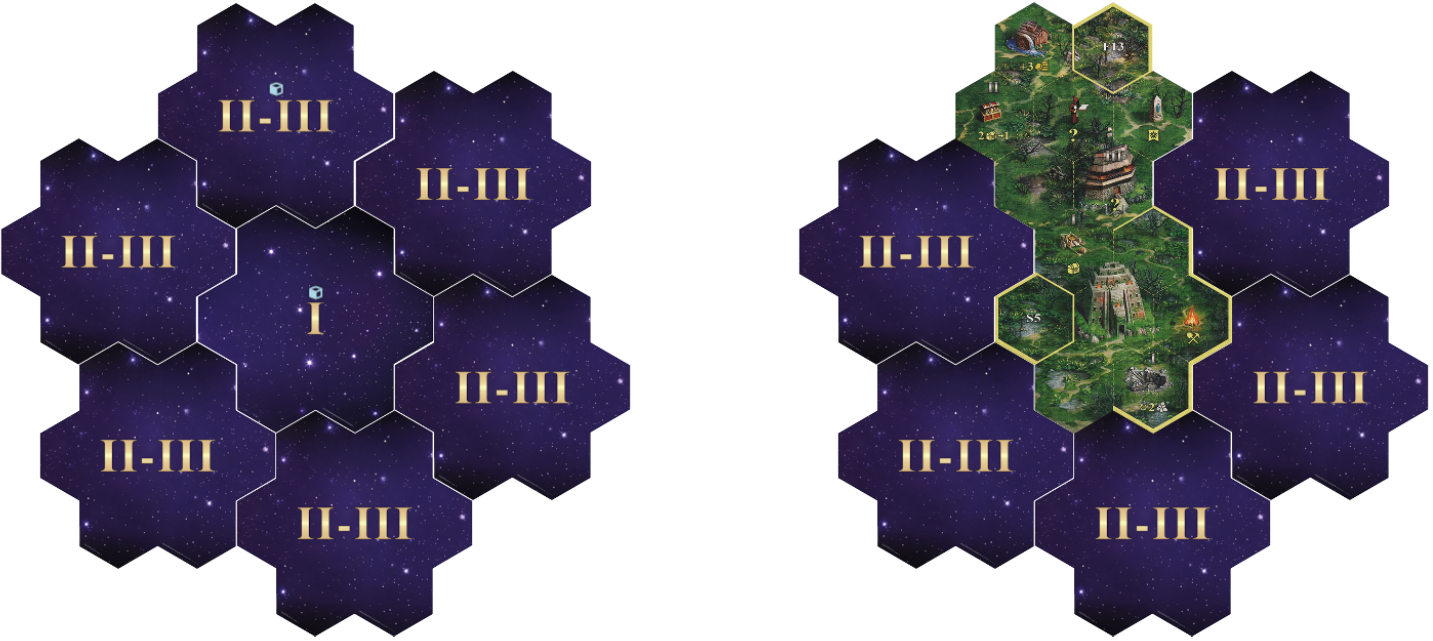
\includegraphics[width=0.68\paperwidth]{\maps/close_to_enemies_p1.png}
  \end{figure}
%   \vspace{2em}
  \begin{figure}[h!]
    \centering
    \captionof{figure}{\textbf{2-PLAYER SCENARIO | EXAMPLE }}
    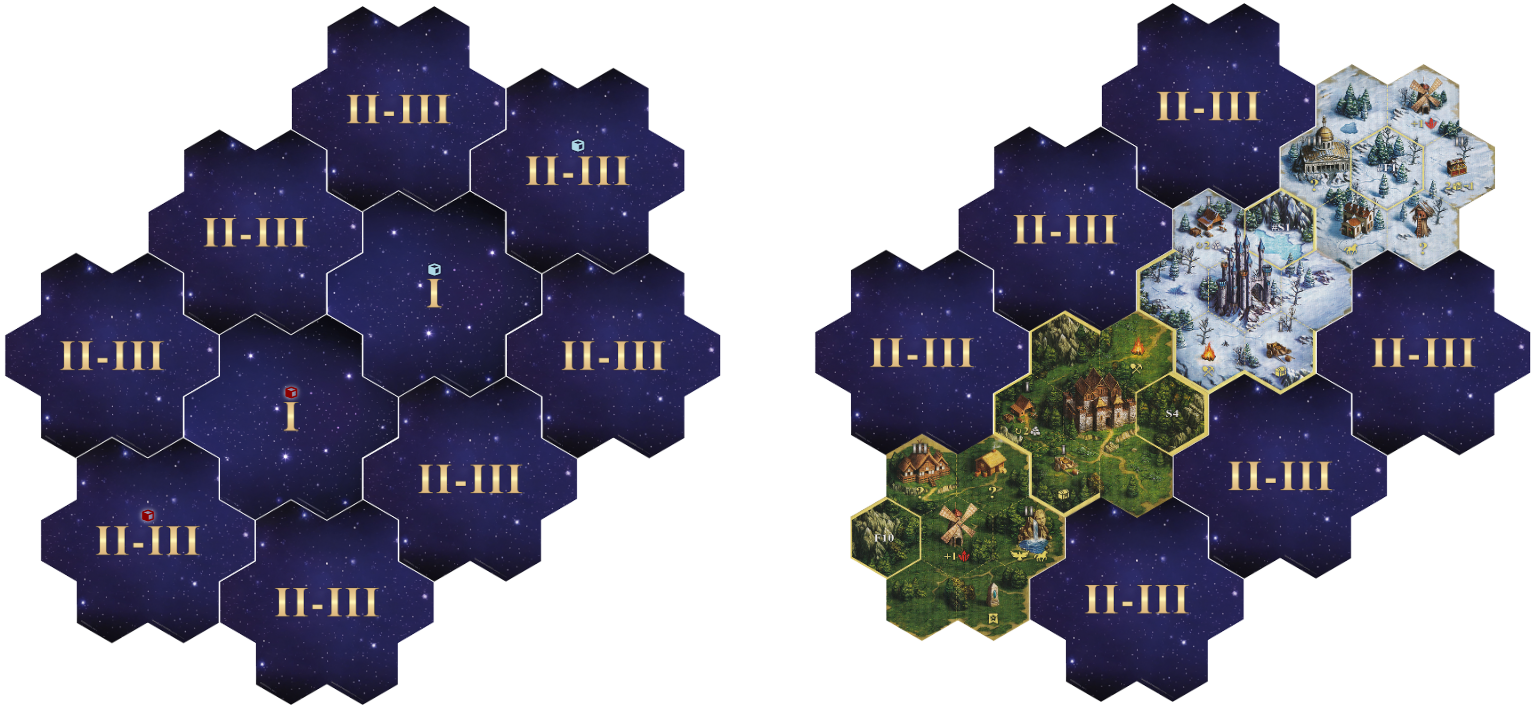
\includegraphics[width=0.68\paperwidth]{\maps/close_to_enemies_p2.png}
  \end{figure}
%   \vspace{2em}
  \begin{figure}[h!]
    \centering
    \captionof{figure}{\textbf{3-PLAYER SCENARIO | EXAMPLE}}
    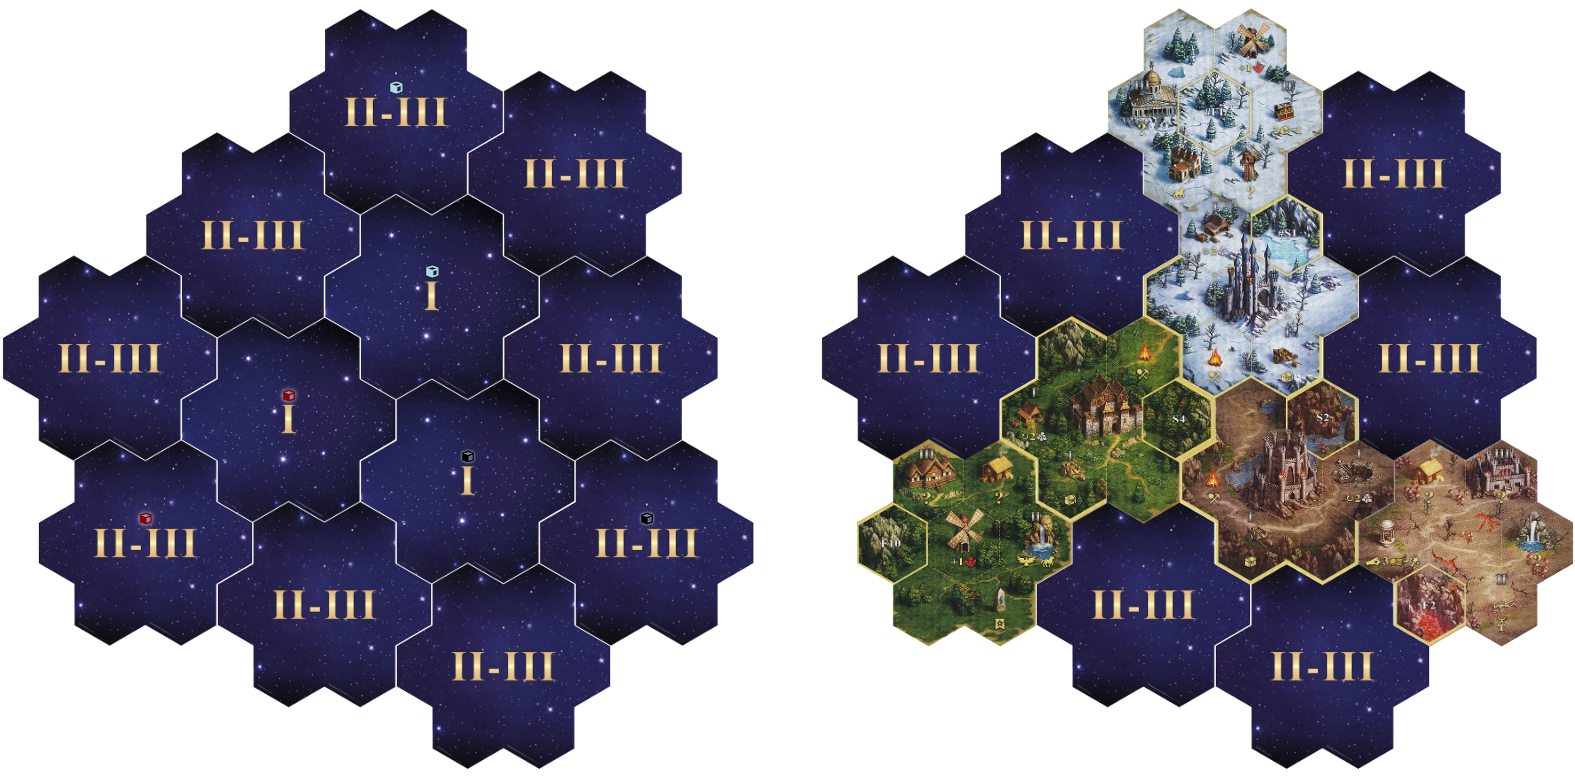
\includegraphics[width=0.75\paperwidth]{\maps/close_to_enemies_p3.png}
  \end{figure}
%   \vspace{2em}
  \begin{figure}[h!]
    \centering
    \captionof{figure}{\textbf{4-PLAYER SCENARIO | EXAMPLE}}
    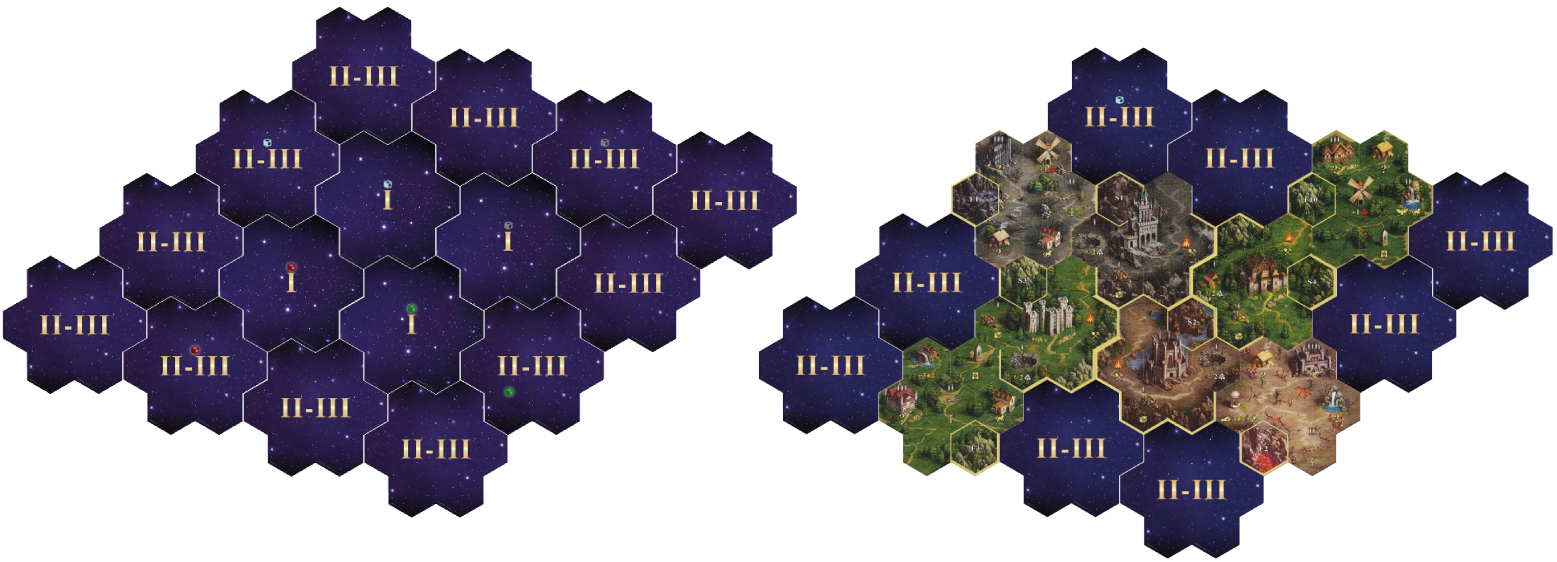
\includegraphics[width=0.85\paperwidth]{\maps/close_to_enemies_p4.png}
  \end{figure}
%   \vspace{2em}
  \begin{figure}[h!]
    \centering
    \captionof{figure}{\textbf{5-PLAYER SCENARIO | EXAMPLE}}
    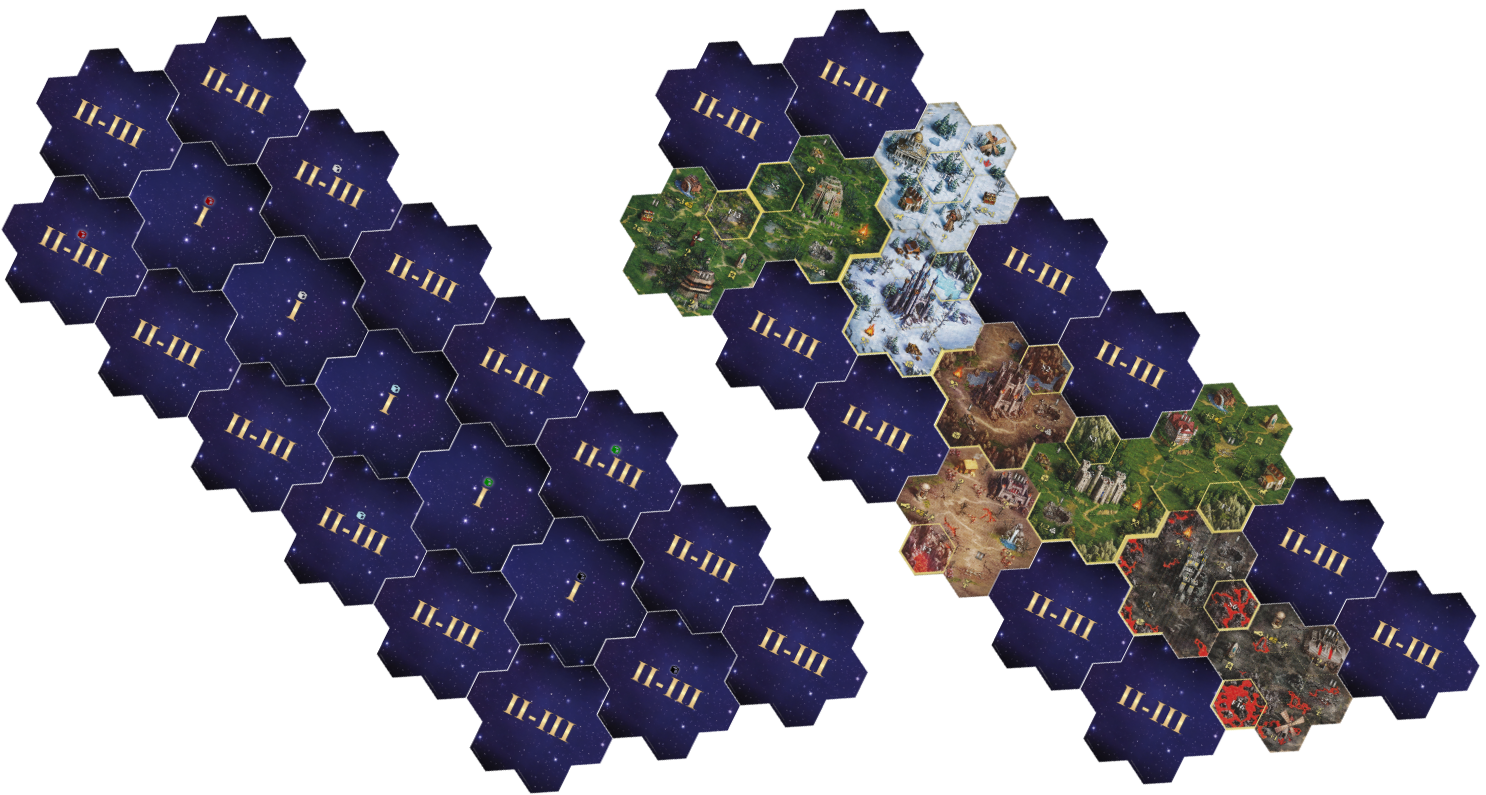
\includegraphics[width=0.75\paperwidth]{\maps/close_to_enemies_p5.png}
  \end{figure}
%   \vspace{2em}
  \begin{figure}[h!]
    \centering
    \captionof{figure}{\textbf{6-PLAYER SCENARIO | EXAMPLE}}
    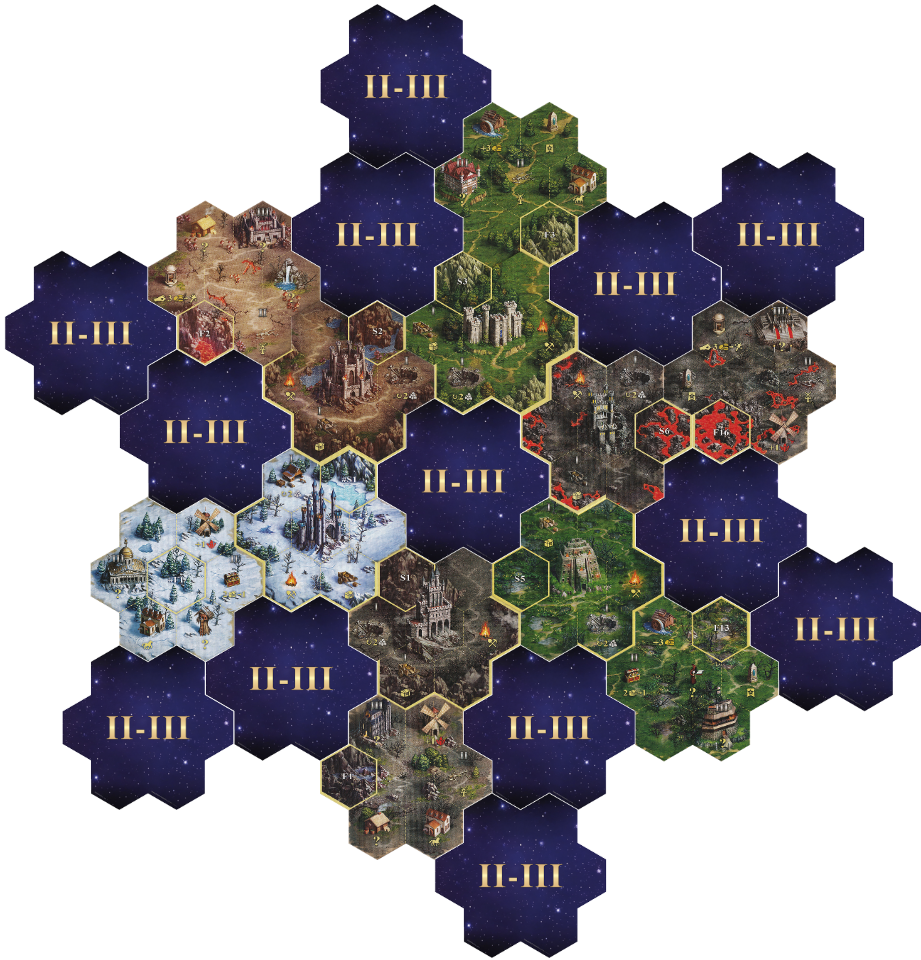
\includegraphics[width=0.75\paperwidth]{\maps/close_to_enemies_p6.png}
  \end{figure}

\end{center}
